\documentclass[12pt]{article}

\usepackage{graphicx}
\usepackage{float}
\usepackage{subfig}

\begin{document}
Motor thrust testing:

\section{Designing the drone body PCB}

The main body of the drone is created as a PCB, so that the body hosts both the structural component and the electrical 
connections of the drone. Since the project formulation's main goals dictates the drones size and mechanical properties, 
the drones size was chosen to be 100 $mm^2$, since this size could accommodate all the needed components of the drone. 
The frame itself was designed in Siemens NX as a simple outline with holes for the motor mounts. 
This outline was exported in a DXF format into Autodesk Eagle were the actual PCB was designed from the needed electrical circuit 
(TO BE EITHER FURTHER DESCRIBED OR 'LINKED' TO HERE). The microcontroller of the drone is mounted by pin headers, 
the motors by the motor mounts and the remaining components by soldering onto the top layer. 
The position of the microcontroller is offset from the center, in order to ensure that the In-built IMU is centered to the exact middle of the PCB.

\begin{figure}[H]%
    \centering
    \subfloat[\centering CAD View]{{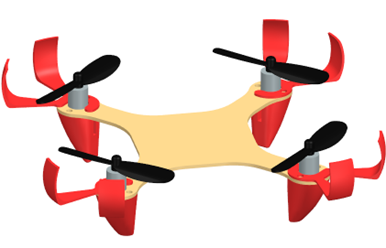
\includegraphics[width=5cm]{DroneCAD.png} }}%
    \qquad
    \subfloat[\centering PCB View]{{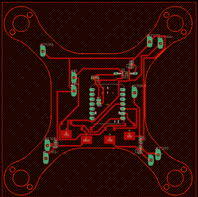
\includegraphics[width=5cm]{PCBpicture.png} }}%
    \caption{Drone model}%
    \label{fig:example}%
\end{figure}

With the combination of the CAD-outline and the electrical schematic, PCB Gerber files could be output for production. The only excess parts needed for the drone would be motor mounts and prop guards (prop guards solely for testing, not for final use).
 The Motor mounts act as both landing legs and motor mounts. They would be designed in order for the motors to press fit into the central hole, 
mounted onto the PCB by screws into the motor mount going through the PCB. The designed mounting parts was printed in PLA on a Prusa MK3S+ 3D printer. 

\begin{figure}[H]%
    \centering
    \subfloat[\centering Motor Mount]{{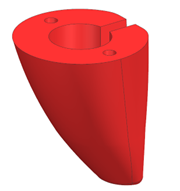
\includegraphics[width=3cm]{Droneleg.png} }}%
    \qquad
    \subfloat[\centering Mounted Motor]{{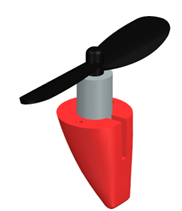
\includegraphics[width=3cm]{Dronepressfit.png} }}%
    \qquad
    \subfloat[\centering Prop Guard]{{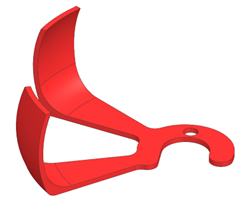
\includegraphics[width=3cm]{Dronepropguard.png} }}%
    \caption{3D-Printed drone parts}%
    \label{fig:example}%
\end{figure}

The project formulation states that the “Stress of the drone’s structural system should not exceed rupture point. System does not experience fracture”. This was tested through Ansys Mechanical Static Structural Analysis. Using the CAD model of the drone, the following boundary conditions were applied: Fixed constraint on the bottom area (excluding the drones arms), Z direction forces (upwards) was applied on each of the motor mount screw holes according to the found motor thrust, a single force vector in the Z direction (downwards) was applied to the top face (excluding the drones arms), to resemble the gravity force caused by the weight of the drone. Besides the boundary condition, the setup contained a mesh refinement of 3 steps, a material assignment of FR4 Fiber Glass Epoxy Board and a solution setting of equivalent stress. Below is a picture of the stress simulation of the initial design, which showed to have clear stress concentrations in the corners where the motor arms runs into the body section. The stress concentration had a magnitude of 1.6839 MPa which is satisfactory regarding the requirement of fracture, since the tensile strength of the given material is 380 MPa FR4 LINK CODE. 

\begin{figure}[H]%
    \centering
    \subfloat{{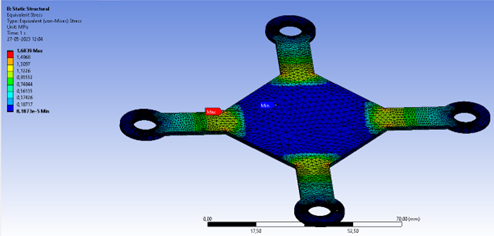
\includegraphics[width=10cm]{Ansys1.png} }}%
    \caption{Initial Ansys Simulation}%
    \label{fig:example}%
\end{figure}

Although it was clear that the drone body would be strong enough to operate under max power, the stress concentrations were undesirable. Therefore 20 mm radii was added to the stress all corner points of the drone body. Repeating the simulation with the same boundary conditions, it was clear that the added radii removed the stress concentrations and instead distributed the stress over a broader area of the motor arms. Furthermore, it was found that the maximum stress was found to be 0.87154 MPa, which is approximately half the maximum strength of the initial model that had the stress concentrations.

\begin{figure}[H]%
    \centering
    \subfloat{{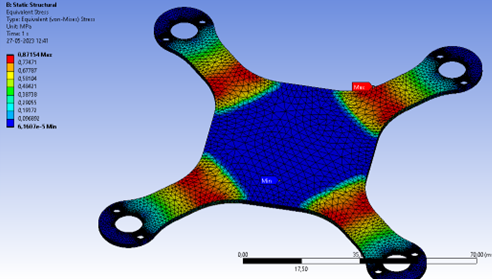
\includegraphics[width=10cm]{Ansys2.png} }}%
    \caption{Final Ansys Simulation}%
    \label{fig:example}%
\end{figure}

\end{document}